\documentclass{beamer}

\usepackage[utf8]{inputenc}
\usepackage{default}

\mode<presentation>
%{ \usetheme{boxes} }


\usetheme{Madrid}

\usepackage{times}
\usepackage{graphicx}
\usepackage{tabulary}
\usepackage{listings}
\usepackage{verbatimbox}
\usepackage{graphicx}
\usepackage{lmodern}
\usepackage[absolute,overlay]{textpos}
\usepackage{pgfpages}
\usepackage{color}
\usepackage{multicol}

\pgfdeclareimage[height=1.0cm]{logo_rcc}{icons/logo_rcc.png}
\setlength{\TPHorizModule}{1mm}
\setlength{\TPVertModule}{1mm}
\newcommand{\RCCLogo}{
\begin{textblock}{14}(1.5,1.5)
  \pgfuseimage{logo_rcc}
\end{textblock}
}


\pgfdeclareimage[height=1.0cm]{tux}{icons/tux.png}
\newcommand{\TUX}{
\begin{textblock}{14}(115.5,1.5)
  \pgfuseimage{tux}
\end{textblock}
}


\definecolor{mycolorcli}{RGB}{53,154,26}
\definecolor{mycolorcode}{RGB}{0,0,255}
\definecolor{mycolordef}{RGB}{255,0,0}
\definecolor{mycolorlink}{RGB}{184,4,255}


\title{\huge{Introduction to Linux \& RCC}}
\author{Igor Yakushin \\ \texttt{ivy2@uchicago.edu}}
%\date{March 31, 2018}

\definecolor{ChicagoMaroon}{RGB}{128,0,0}

\setbeamercolor{title}{bg=ChicagoMaroon}

\begin{document}

\setbeamertemplate{navigation symbols}{}

\setbeamercolor{fcolor}{fg=white,bg=ChicagoMaroon}
\setbeamertemplate{footline}{
\begin{beamercolorbox}[ht=4ex,leftskip=1.4cm,rightskip=.3cm]{fcolor}
\hrule
\vspace{0.1cm}
   \hfill \insertshortdate \hfill \insertframenumber/\inserttotalframenumber
\end{beamercolorbox}
}

\setbeamercolor{frametitle}{bg=ChicagoMaroon,fg=white}

\begin{frame}
%\RCCLogo
\TUX
\titlepage
\end{frame}

\section{Where to get this tutorial}
\begin{frame}[fragile]
  \frametitle{Where to get this tutorial}
  \begin{itemize}
  \item Point your browser to  {\color{mycolorcli}\verb|https://github.com/igory1999/Linux|}
  \end{itemize}
\end{frame}

\section{History}
\begin{frame}[fragile]
  \frametitle{History}
  \begin{itemize}
  \item UNIX operating system, the commercial ancestor of Linux, was developed by Ken Thompson and Dennis Ritchie at AT\&T Bell Labs in 1969 and released in 1970
\begin{center}
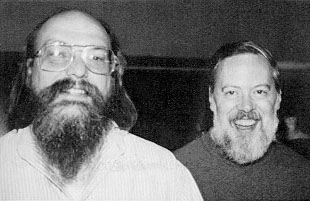
\includegraphics[width=3cm]{graphs/Ken_n_dennis.jpg}
\end{center}
  \item Later several more commercial UNIX distributions appeared
  \item In 1983, Richard Stallman started the GNU project with the goal of creating a free UNIX-like operating system.
\begin{center}
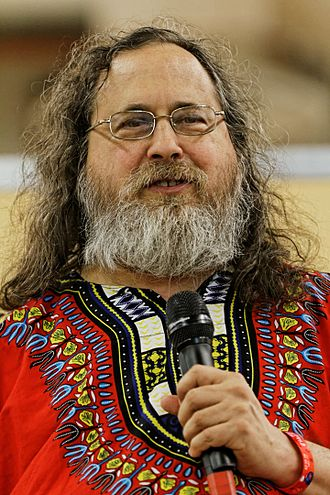
\includegraphics[width=2cm]{graphs/Richard_Stallman.jpg}
\end{center}
\end{itemize}
\end{frame}

\begin{frame}[fragile]
  \frametitle{History}
  \begin{itemize}
  \item By the early 1990s, there was almost enough available software to create a full operating system. However, the GNU kernel did not work out.
  \item In 1991, while studying computer science at University of Helsinki, Linus Torvalds, at the age of 21, began a project that later became the Linux kernel
\begin{center}
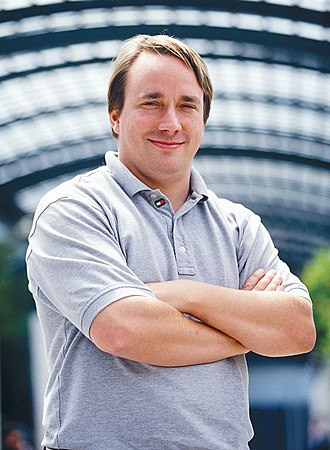
\includegraphics[width=2cm]{graphs/Linus_Torvalds.jpeg}
\end{center}
  \item GNU/Linux provided free open source UNIX environment without expensive license fees
  \item Nowadays GNU/Linux is usually just called Linux
  \end{itemize}
\end{frame}


\begin{frame}[fragile]
  \frametitle{History}
  \begin{itemize}
  \item It is free, open source and a lot of developers and companies from all around the world keep contributing to Linux kernel and application software
  \item When I started using Linux in 1994, it felt almost illegal: 
    \begin{itemize}
    \item your employer would typically be very suspicious if you are not using the blessed Windows 
    \item no vendors would talk to you if you say you need their hardware to behave under Linux
    \item due to no vendor support one had to be very careful when buying hardware to make sure that all the components would work with Linux 
    \item it was quite an adventure to install it
    \item many useful applications were not available under Linux and one had to use Windows for those
    \end{itemize}
  \item These days Linux is the mainstream server platform, it is used on almost all HPC sites, embedded devices, etc.
  \item It is used by such companies as Google, Facebook, Oracle, banks from Wall Street, etc.
  \end{itemize}
\end{frame}

\begin{frame}[fragile]
  \frametitle{History}
  \begin{itemize}
  \item Even Microsoft these days relies on Linux in their Azure cloud platform and is one of the major contributors to Linux
  \item There is a good vendor support now, especially for servers and HPC systems, although still not necessarily for consumer laptops/desktops
  \item There are free and commercial applications to do anything under Linux and since the beginning of the century I use Linux for everything and have no use for Windows
  \item It is easy to install Linux today
  \item There are hundreds distributions to select from: Debian, RedHat, Scientific Linux, Fedora, Slackware, Gentoo, etc.
  \item Two big families of distributions: Debian-based and RedHat-based
  \item For a typical user it is recommended to start with one of the most popular distributions: for example, Ubuntu or CentOS - huge user community, easy to find answers to your questions, more free and commercial 
    software works out of the box, more frequent updates, security patches are available
  \end{itemize}
\end{frame}


\begin{frame}[fragile]
  \frametitle{History}
  \begin{itemize}
  \item If you want to install Linux and start experimenting with it, the easiest thing to do is to install VirtualBox (https://www.virtualbox.org ) 
    which is available for all the major OSes (Windows, MacOS, Linux) and install Linux as a virtual machine before you are ready to put it on bare hardware
  \item That way you can quickly experiment with various Linux distributions without having to wipe out the existing OS
  \item $99\%$ of this talk applies to Mac as well even though one can completely avoid command line by using GUI. MacOS is also based on UNIX and its command line is not that much different from Linux.
  \item Strictly speaking you can get away today with using Linux via GUI and not dealing with command line, at least on your desktop/laptop but not on HPC clusters. However, using command line, once you get used to it,
    is actually easier and gives you more power so it is worth learning it.
\end{itemize}
\end{frame}


\section{Login to midway}

\subsection{Login to midway: ssh}
\begin{frame}[fragile]
  \frametitle{Login to midway: ssh}
  \begin{itemize}
  \item A standard way to login to a remote Linux machine is to use {\color{mycolorcli}ssh} - {\color{mycolordef}s}ecure {\color{mycolordef}sh}ell. For example, to log into RCC's midway 2 cluster:
{\color{mycolorcli}
\begin{verbatim}
ssh -Y <youruserid>@midway2.rcc.uchicago.edu
\end{verbatim}
}
  \item The {\color{mycolorcli}\verb|-Y|} option allows to use not only command line interface (CLI) but also graphics (\verb|X-windows|) remotely - {\color{mycolordef}X-forwarding}
  \item This assumes that you have ssh client on your laptop.
  \item If you run Linux on your laptop, you have everything but then you probably would not be here
  \item If you use Mac, than you should have ssh client although for X-forwarding you might need to install X11 server and client libraries, 
    which can be downloaded from the XQuartz project page: {\color{mycolorcli}\verb|https://www.xquartz.org|}
  \end{itemize}
\end{frame}

\begin{frame}[fragile]
  \frametitle{Login to midway: ssh}
  \begin{itemize}
  \item If you have MS Windows, you might need to install a client. For example:
    \begin{itemize}
    \item Putty: 
      \begin{itemize}
      \item {\color{mycolorcli}\verb|http://www.putty.org|}
      \item considered standard ssh client under MS Windows
      \item does not allow X-forwarding
      \end{itemize}
    \item Bitvise:
      \begin{itemize}
      \item {\color{mycolorcli}\verb|http://www.putty.org|}
      \item more advanced than Putty, available from the same page
      \item does not allow X-forwarding
      \end{itemize}
    \item Cygwin:
      \begin{itemize}
      \item {\color{mycolorcli}\verb|http://www.cygwin.org|}
      \item allows you to run most UNIX commands inside MS Windows - might be too much if you just want ssh client
      \item contrary to the above ssh clients for Windows, it allows X-forwading if you install X11 server
      \item It might take several hours and gigabytes to install the full Cygwin distribution but it can include everything: C/C++ compilers, python, perl, MySQL and Postgres databases, etc.
      \end{itemize}
    \end{itemize}
  \end{itemize}
\end{frame}


\begin{frame}[fragile]
  \frametitle{Login to midway: ssh}
\begin{itemize}
  \item MobaXterm:
    \begin{itemize}
      \item {\color{mycolorcli}\verb|https://mobaxterm.mobatek.net|}
      \item allows X-forwarding
    \end{itemize}
  \item If you have Chromebook, or anything else running Chrome web browser, you can use ssh extension to Chrome 
    \begin{itemize}
    \item does not allow X-forwarding
    \item should work on any OS if it has Chrome
    \end{itemize}
\end{itemize}
\end{frame}


\subsection{Login to midway: ThinLinc}
\begin{frame}[fragile]
  \frametitle{Login to midway: ThinLinc}
  \begin{itemize}
  \item ThinLinc is portable on the client side in the sense that it should work with any OS on your laptop as long as you have a web browser. For many OSes you can also install client.
  \item It does not work with yubikeys
  \item ThinLinc server is a commercial product that might be running on some Linux sites but is not a standard part of Linux, contrary to ssh server, 
    and is not used in most other places. At RCC we run it on midway 1 \& 2 clusters but not on Hadoop cluster.
  \item So eventually you would need to get used to ssh anyway.
  \end{itemize}
\end{frame}

\begin{frame}[fragile]
  \frametitle{Login to midway: ThinLinc}
  \begin{itemize}
    \item There are two ways to connect with ThinLinc to midway:
      \begin{itemize}
        \item Just use a web browser interface by pointing your browser to {\color{mycolorcli}\verb|https://midway2.rcc.uchicago.edu|}. 
          This might not work well for all browsers, you might have to try several: Chrome, Firefox, Safari...
        \item Install ThinLinc client from {\color{mycolorcli}\verb|https://www.cendio.com/thinlinc/download|}. 
          \begin{itemize}
          \item Configure the client to connect to {\color{mycolorcli}\verb|midway2.rcc.uchicago.edu|}
          \item You can specify the dimensions of the window in which it is running. I am usually using full screen.
          \item It does X-forwarding and you can use graphics, usually it works faster than vanilla ssh.
          \item The client has trouble with emacs key sequences, web interface does not.
          \end{itemize}
      \end{itemize}
  \end{itemize}
\end{frame}


\subsection{Login to midway: JupyterHub}
\begin{frame}[fragile]
  \frametitle{Login to midway: JupyterHub}
  \begin{itemize}
  \item Yet another non-standard  but free way to log into midway cluster is to use JupyterHub.
  \item There are two JupyterHub servers that you can use:
    \begin{itemize}
      \item {\color{mycolorcli}\verb|https://jupyter.rcc.uchicago.edu|} - midway 1
      \item {\color{mycolorcli}\verb|https://hadoop.rcc.uchicago.edu|} - Hadoop 
    \end{itemize}
    \item Just point your browser and use your midway username and password
    \item JupyterHub, besides running notebooks in python, R, and other interpreters, gives you a terminal and an ability to upload/download files
    \item It does not allow X-forwarding
    \item Since all RCC clusters share home file system, everything uploaded via any of the above JupyterHub instances becomes accessible from all the clusters
    \item There is no JupyterHub on midway 2 but once you get to a terminal, you can ssh there if necessary.
  \end{itemize}
\end{frame}


\subsection{Login to midway: 2fa}
\begin{frame}[fragile]
  \frametitle{Login to midway: 2fa}
  \begin{itemize}
  \item Since the end of last year, there is an extra extremely annoying security complication: {\color{mycolordef}2-factor authentication}.
  \item You need to follow the instructions on {\color{mycolorcli}\verb|https://cnet.uchicago.edu/2FA/index.htm|} to enroll in 2-factor authentication. 
Another useful related page: {\color{mycolorcli}\verb|https://2fa.rcc.uchicago.edu|}.
  \item You would need to install an application on your phone so that when you try to connect to midway, you get notification on your phone to which you need to respond
  \item If you do not have a phone or travelling abroad, you can get a set of passcodes that you can type instead, each time using the next passcode from the list and periodically 
    getting a new list once you use all the numbers from there.
  \end{itemize}
\end{frame}


\subsection{Lab 1}
\begin{frame}[fragile]
  \frametitle{Lab 1: connect to midway 2}
  \begin{itemize}
  \item Connect to midway 2 using one or more of the described methods, if possible with X-forwarding 
    \begin{itemize}
    \item 15 minutes or as much time as necessary for everbody to get onto midway 2 since the rest of the tutorial relies on your ability to
    execute commands there.
    \end{itemize}

    \item Once you are on midway, get the presentation and labs from git repo:
{\small
{\color{mycolorcli}
\begin{verbatim}
git clone https://github.com/igory1999/Linux.git
\end{verbatim}
}
}

  \end{itemize}
\end{frame}

\section{Navigating the file system}
\subsection{Directory tree}
\begin{frame}[fragile]
  \frametitle{Navigating the file system: directory tree}
\begin{itemize}
\item Linux, like any other OS I have seen so far, organizes directories and files into a tree
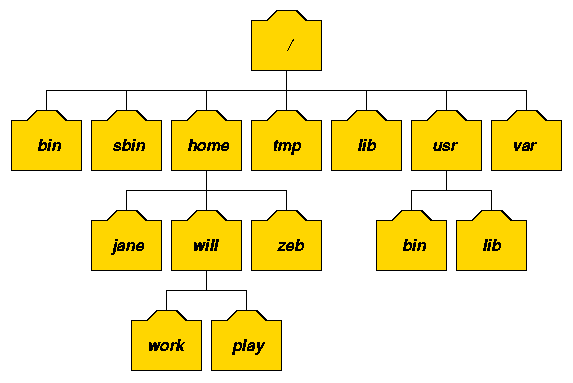
\includegraphics[width=6cm]{graphs/tree.png}
\item At the top of the tree there is root {\color{mycolorcli}\verb|/|}
\item The linux system commands, like ls, cp, mv, are typically in {\color{mycolorcli}\verb|/bin|}
\item Application programs, like emacs, vi, find, are typically in {\color{mycolorcli}\verb|/usr/bin|}
\item Commands for system administrators are usually in {\color{mycolorcli}\verb|/sbin|}
\item Libraries are usually in {\color{mycolorcli}\verb|/lib|}, {\color{mycolorcli}\verb|/lib64|}, {\color{mycolorcli}\verb|/usr/lib|}
\item User home directories are under {\color{mycolorcli}\verb|/home|}
\item Home directory of the root (system administrator user) is in {\color{mycolorcli}\verb|/root|}
\end{itemize}
\end{frame}

\begin{frame}[fragile]
  \frametitle{Navigating the file system: directory tree}
  \begin{itemize}
  \item Many programs write temporary files into {\color{mycolorcli}\verb|/tmp|}
  \item Various services often keep log files in {\color{mycolorcli}\verb|/var/log|}
  \item Configuration files for the system and various services are typically under {\color{mycolorcli}\verb|/etc|}
  \item To refer to a particular directory you can either use {\color{mycolordef}\verb|absolute path|} or {\color{mycolordef}\verb|relative path|}:
    \begin{itemize}
    \item When using an absolute path, you construct it from the top of the directory tree. For example: {\color{mycolorcli}\verb|/home/ivy2/dir1/dir2/dir3|}
    \item When using a relative path, you construct it from your current location. 
      \begin{itemize}
      \item For example, if you are in {\color{mycolorcli}\verb|/home/ivy2/dir1|} you can refer to the above directory as 
        {\color{mycolorcli}\verb|dir2/dir3|}. 
      \item If you are already in {\color{mycolorcli}\verb|/home/ivy2/dir1/dir2/dir3|}, you can refer to the current directory as  {\color{mycolorcli}\verb|.|}. Sometimes it is necessary: for example,
        when you want to execute a program from the current directory and do not have {\color{mycolorcli}\verb|.|} in {\color{mycolorcli}\verb|$PATH|}: {\color{mycolorcli}\verb|./myprogram|}. 
      \item If you are in  {\color{mycolorcli}\verb|/home/ivy2/dir4/dir5/dir6|}, you refer to the above directory as {\color{mycolorcli}\verb|../../../dir1/dir2/dir3|}.  {\color{mycolorcli}\verb|..|} denote a
        parent directory.
      \end{itemize}
    \end{itemize}
  \end{itemize}
\end{frame}


\begin{frame}[fragile]
  \frametitle{Navigating the file system: directory tree}
  \begin{itemize}
  \item To list what files and subdirectories are in a particular directory and learn their properties, such as size, permissions, ownership, last date of modification, use {\color{mycolorcli}\verb|ls|}
  \item To change directory, use {\color{mycolorcli}\verb|cd|}
  \item To see what directory you are in, use {\color{mycolorcli}\verb|pwd|}
  \item To make directory, use {\color{mycolorcli}\verb|mkdir|}
  \item To remove a file or directory, use {\color{mycolorcli}\verb|rm|}
  \item To create an empty file, for example, for testing purposes, {\color{mycolorcli}\verb|touch|}
  \item To find a file or directory under some subtree, use {\color{mycolorcli}\verb|find|} 
  \item To find an exact syntax, options, try {\color{mycolorcli}man} or {\color{mycolorcli}\verb|--help|} option.
  \end{itemize}
\end{frame}


\subsection{Lab 2}
\begin{frame}[fragile]
  \frametitle{Navigating the file system: Lab 2}

\begin{itemize}
\item
{\color{mycolorcli}
\begin{verbatim}
cd $HOME/Linux/labs/2
\end{verbatim}
}
\item Follow instructions in {\color{mycolorcli}\verb|README.md|}
\end{itemize}

\end{frame}

\section{File editing}
\subsection{emacs}
\begin{frame}[fragile]
  \frametitle{File editing: emacs}
\begin{itemize}
\item {\color{mycolorcli}\verb|emacs [<filename>]|} starts GUI version if X is forwarded, otherwise, it either starts terminal version or complains
\item {\color{mycolorcli}\verb|emacs -nw [<filename>]|} starts terminal version
\item Just type your text
\item To cut everything from the current character to the end of line: {\color{mycolorcli}\verb|Ctrl+k|}
\item To paste: {\color{mycolorcli}\verb|Ctrl+y|}
\item To save a file: {\color{mycolorcli}\verb|Ctrl+x Ctrl+s|}
\item To save and exit: {\color{mycolorcli}\verb|Ctrl+x Ctrl+c|}
\item To mark a big part of text, {\color{mycolorcli}\verb|Esc Shift+@|}, move cursor, do something with the selected text, for example {\color{mycolorcli}\verb|Ctrl+w|} to cut it.
\item To search text forward for some string {\color{mycolorcli}\verb|Ctrl+s|}, to search backward {\color{mycolorcli}\verb|Ctrl+r|}
\item To move cursor to the end of the line {\color{mycolorcli}\verb|Ctrl+e|}, to move cursor to the beginning of the line {\color{mycolorcli}\verb|Ctrl+a|}
\end{itemize}
\end{frame}

\begin{frame}[fragile]
  \frametitle{File editing: emacs}
\begin{itemize}
\item To replace a string starting from the current character till the end of file: {\color{mycolorcli}\verb|Esc+x replace-string|}, type source and target.
\item You can open several files inside emacs and keep switching between different buffers, copying and pasting between different files.
\item To open an existing file or start a new one in emacs {\color{mycolorcli}\verb|Ctrl+x Ctrl+f|}
\item To list open files (buffers): {\color{mycolorcli}\verb|Ctrl+x Ctrl+b|}
\item To switch between different buffers: {\color{mycolorcli}\verb|Ctrl+x b|}
\item One can open multiple windows, each looking at the same or different buffers.
\item To open a new window below:  {\color{mycolorcli}\verb|Ctrl+x 2|}
\item To open a new window to the right:  {\color{mycolorcli}\verb|Ctrl+x 3|}
\item To remove other windows: {\color{mycolorcli}\verb|Ctrl+x 1|}
\item To move to other window: {\color{mycolorcli}\verb|Ctrl+x o|}
\item One can cancel a command in construction with  {\color{mycolorcli}\verb|Ctrl+g|}
\end{itemize}
\end{frame}


\begin{frame}[fragile]
  \frametitle{File editing: emacs}
\begin{itemize}
\item By default emacs shows line number on the bottom bar. One can ask it to show also column number with {\color{mycolorcli}\verb|Esc+x column-number-mode|}
\item To undo, {\color{mycolorcli}\verb|Ctrl+x u|}
\item There are thousands of other commands and options but the above is typically enough for \verb|99%| of text editing
\item You can define your own macros
\item Emacs usually detects what language you are programming in and formats text accordingly. It can recognize C, C++, Fortran, Python,
Java, HTML, LaTeX, etc. Language specific menu appears in GUI version of emacs.
\item The other popular editor in Linux which we do not discuss here is {\color{mycolorcli}\verb|vi|}. 
\item There are many other higher level and more user friendly editors like {\color{mycolorcli}gedit}, 
  nano, lyx, libreoffice, atom, etc. 
  but you better know either emacs or vi since those are available everywhere.
\end{itemize}
\end{frame}


\subsection{emacs}
\begin{frame}[fragile]
  \frametitle{File editing: gedit}
  \begin{itemize}
  \item If you do not want to spend a few hours to get used to the power of emacs, just use
    {\color{mycolorcli}gedit}
  \item It has similar intuitive GUI interface to Window's notebook, nothing to learn
  \item However, you need either to use ssh client that does X-forwarding or use ThinLinc
  \end{itemize}
\end{frame}


\subsection{Lab 3}
\begin{frame}[fragile]
  \frametitle{File editing: Lab 3}

\begin{itemize}
\item
{\color{mycolorcli}
\begin{verbatim}
cd ~/Linux/labs/3
\end{verbatim}
}
\item Follow instructions in {\color{mycolorcli}\verb|README.md|} file

\end{itemize}
\end{frame}


\section{Copying and moving files and folders}
\begin{frame}[fragile]
  \frametitle{Copying and moving files and folders}
\begin{itemize}
\item To copy files on a Linux system, use {\color{mycolorcli}\verb|cp|}, to copy folders, use either {\color{mycolorcli}\verb|cp -r|} or {\color{mycolorcli}\verb|rsync -av|}
\begin{itemize}
\item {\color{mycolorcli}\verb|cp <fromfile> <tofile>|}
\item {\color{mycolorcli}\verb|cp -r <fromdirectory> <todirectory>|}
\item {\color{mycolorcli}\verb|mv <fromfile> <tofile>|}
\item {\color{mycolorcli}\verb|rsync -av <fromdirectory> <todirectory>|}
\end{itemize}
\item {\color{mycolorcli}\verb|rsync|}, contrary to {\color{mycolorcli}\verb|cp|}, is restartable, if it is interrupted in the middle and you start it again, it figures out what has already been done and picks up where it left.
\item To copy file/directory to remote host, if you have ssh client, do
{\tiny
{\color{mycolorcli}
\begin{verbatim}
scp <fromfile> <yourusername>@midway2.rcc.uchicago.edu:<tofile>
scp -r <fromdirectory> <yourusername>@midway2.rcc.uchicago.edu:<todirectory>
rsync -av <fromdirectory> <yourusername>@midway2.rcc.uchicago.edu:<todirectory>
\end{verbatim}
}
}
\item To copy file/directory from remote host, if you have ssh client, do
{\tiny
{\color{mycolorcli}
\begin{verbatim}
scp <yourusername>@midway2.rcc.uchicago.edu:<fromfile> <tofile>
scp -r <yourusername>@midway2.rcc.uchicago.edu:<fromdirectory> <todirectory>
rsync -av  <yourusername>@midway2.rcc.uchicago.edu:<fromdirectory> <todirectory>
\end{verbatim}
}
}
\item {\color{mycolorcli}\verb|rsync|} uses {\color{mycolorcli}\verb|ssh|} underneath unless {\color{mycolorcli}\verb|rsync|} server is running on the remote site
\end{itemize}
\end{frame}


\begin{frame}[fragile]
  \frametitle{Copying and moving files and folders}
\begin{itemize}
\item If you have a lot of data to copy between your laptop and midway or between midway and some other Globus end point, use Globus. For instructions, see 
{\color{mycolorcli}
\begin{verbatim}
https://globus.rcc.uchicago.edu/globus-app
\end{verbatim}
}
\item If ssh/scp still does not work for you, you can use JupyterHub to upload/download data to/from midway
{\color{mycolorcli}
\begin{verbatim}
https://jupyter.rcc.uchicago.edu
\end{verbatim}
}
\item If you are transferring text files from Windows/Mac to Linux or the other way arround, you might need to run {\color{mycolorcli}\verb|dos2unix|} or {\color{mycolorcli}\verb|unix2dos|} on those files 
  since the end of line character in Linux and Windows/Mac text files is different which might cause problems for some programs. 
\end{itemize}
\end{frame}

\begin{frame}[fragile]
  \frametitle{Copying and moving files and folders}
\begin{itemize}
\item Compare,  using {\color{mycolorcli}\verb|cat -A <filename> |}, the same text file edited on Windows and Linux
  \begin{itemize}
  \item {\color{mycolorcli}\verb|windows.txt|}:
\begin{verbatim}
one two^M$
three^Ifour^M$
\end{verbatim}
  \item {\color{mycolorcli}\verb|linux.txt|}:
\begin{verbatim}
one two$
three^Ifour$
\end{verbatim}
  \end{itemize}
\item  {\color{mycolorcli}\verb|cat -A <filename> |} displays non-printable characters denoting them in some way. For example, {\color{mycolorcli}\verb|^I|} means tab, {\color{mycolorcli}\verb|$|} - Linux end of line character.
\item Look at the end of the lines. In Windows there is an extra \verb|^M| before \verb|$|.
\item To convert Windows end of line character to Linux, run {\color{mycolorcli}\verb|dos2unix windows.txt|}
\end{itemize}
\end{frame}



\subsection{Lab 4}
\begin{frame}[fragile]
  \frametitle{Lab 4}
\begin{itemize}
\item
{\color{mycolorcli}
\begin{verbatim}
cd $HOME/Linux/labs/4
\end{verbatim}
}
\item Follow instructions in {\color{mycolorcli}\verb|README.md|}
\end{itemize}

\end{frame}


\section{File and directory permissions}
\begin{frame}[fragile]
  \frametitle{File and directory permissions}
  \begin{itemize}
    \item For each file or directory you can set who can 
      \begin{itemize}
      \item {\color{mycolordef}r} - read
      \item {\color{mycolordef}w} - write
      \item {\color{mycolordef}x} - execute (or browse for directory)
      \end{itemize}
      it.
    \item For permissions purposes, there are four types of ``who'':
      \begin{itemize}
      \item {\color{mycolordef}u} - user
      \item {\color{mycolordef}g} - group
      \item {\color{mycolordef}o} - others
      \item {\color{mycolordef}a} - all
      \end{itemize}
    \item There is ACL (access control list) that gives finer control over permissions but I had never any reason to use it so far.
    \item There are permissions that each file and directory gets by default. The default is configurable.
  \end{itemize}
\end{frame}

\begin{frame}[fragile]
  \frametitle{File and directory permissions}
  \begin{itemize}
    \item You can see permissions with  {\color{mycolorcli}ls -l}:
{\color{mycolorcli}
\begin{verbatim}
ls -l t8
-rwxrw-r-x 2 ivy2 kicp 243640 Dec 11 09:38 t8
\end{verbatim}
}      
The above says that a file {\color{mycolorcli}\verb|t8|} was last modified on  {\color{mycolorcli}\verb|Dec 11 09:38|}, has  {\color{mycolorcli}\verb|243640|} bytes, belongs to  
{\color{mycolorcli}\verb|ivy2|} user and  {\color{mycolorcli}\verb|kicp|} group (often default group is same as username), 
has only two hardware links to it, is a file (for directory the first character would be  {\color{mycolorcli}\verb|d|}, for symbolic links it is    
{\color{mycolorcli}\verb|l|}), has  {\color{mycolorcli}\verb|rwx|} permissions for user,  {\color{mycolorcli}\verb|rw-|} permissions for the group,  {\color{mycolorcli}\verb|r-x|} permissions for others.
\item The executable permission on a file means that it can be used as a program.
\item The executable permission on a directory means that one can go there.
\end{itemize}
\end{frame}


\begin{frame}[fragile]
  \frametitle{File and directory permissions}
  \begin{itemize}
\item To change permissions:
{\color{mycolorcli}
\begin{verbatim}
chmod u-w t8
chmod -R a+X dir1
\end{verbatim}
}
\item The above would remove write permissions for the user and makes 
all directories under {\color{mycolorcli}dir1} browsable by everybody. If one used 'x' instead of 'X', all the files under {\color{mycolorcli}dir1} in addition would become executable. 
\item The ownership of the file/directory is changed with {\color{mycolorcli}chown} but as a user you have rather limited freedom to do it. Only root can change user ownership. You can change group ownership to one of the groups of which you are
  a member:
{\color{mycolorcli}
\begin{verbatim}
chown ivy2:rcc-hadoop t8
\end{verbatim}
}
\item You can find to which groups you belong by executing {\color{mycolorcli}groups} (standard Linux command) or {\color{mycolorcli}\verb|rcchelp user <username>|} (local RCC script)
\end{itemize}
\end{frame}



\section{Bash shell}
\begin{frame}[fragile]
  \frametitle{Bash shell}
\begin{itemize}
\item When you log into Linux, you get into shell - command line interface (CLI) to Linux - where you can type commands and the shell would interpret and execute them. 
\item By default it is {\color{mycolorcli}\verb|bash|}. 
\item There are other shells that you can select: {\color{mycolorcli}\verb|csh|}, {\color{mycolorcli}\verb|tcsh|}, {\color{mycolorcli}\verb|zsh|}, etc.  They mostly differ in syntax but have similar functionality.
\item bash configuration is defined in the following files in your home directory: {\color{mycolorcli}\verb|.bash_profile|}, {\color{mycolorcli}\verb|.bashrc|}, {\color{mycolorcli}\verb|.bash_aliases|}
\item There you can set environmental variables, aliases, define, for example, how your shell prompt looks like, etc.
\item If you start typing a command or a path in shell and press {\color{mycolorcli}TAB}, the shell tries to
  autocomplete
\item {\color{mycolorcli}\verb|history|} shows the previous commands, {\color{mycolorcli}arrow-up}
  returns the previous command if you want to repeat it
\item bash understands many of emacs key combinations: {\color{mycolorcli}\verb|Ctrl+A|},
  {\color{mycolorcli}\verb|Ctrl+E|}
\item Shell can be used as a programming language to write scripts
\end{itemize}
\end{frame}

\section{Environment}
\begin{frame}[fragile]
  \frametitle{Environment}
\begin{itemize}
\item When you type the name of the executable program in a shell, it is looking for it among the paths listed in {\color{mycolorcli}\verb|$PATH|} environmental variable. For example:
{\color{mycolorcli}
\begin{verbatim}
$ echo $PATH
/bin:/software/slurm-current-el7-x86_64/bin:\
/usr/local/bin:/usr/bin:/usr/local/sbin:/usr/sbin:\
\end{verbatim}
}
\item If you have a program in some non-standard location {\color{mycolorcli}\verb|/yet/another/path/bin/myprogram|}, you need to prepend/append another path to {\color{mycolorcli}\verb|PATH|} or use the full path to the executable:
{\color{mycolorcli}
\begin{verbatim}
$ /yet/another/path/bin/myprogram
$ export PATH=/yet/another/path/bin:$PATH
$ myprogram
\end{verbatim}
}
\item To find out where your program is, if its location is in {\color{mycolorcli}\verb|$PATH|}:
{\color{mycolorcli}
\begin{verbatim}
$ which gcc
/usr/bin/gcc
\end{verbatim}
}
\end{itemize}
\end{frame}

\begin{frame}[fragile]
  \frametitle{Environment}
\begin{itemize}
\item Notice that bash would go over the list of paths in order specified and will pick the first available executable with the given name it can find and stop looking after that. 
Therefore, it might make difference if you prepend or append paths.
\item Most of the programs in Linux are dynamically compiled, 
in the sense that they load the necessary libraries at runtime rather then including them into the executable. 
If the library you are using is not at some standard location like
{\color{mycolorcli}\verb|/lib64|}, {\color{mycolorcli}\verb|/usr/lib|}, {\color{mycolorcli}\verb|/usr/lib64|}, 
{\color{mycolorcli}\verb|/usr/local/lib|}, etc, you need to prepend/append the corresponding path to {\color{mycolorcli}\verb|$LD_LIBRARY_PATH|} environmental variable.
\item To see what libraries are loaded or not found for a particular executable:
{\tiny
{\color{mycolorcli}
\begin{verbatim}
$ ldd `which gcc`
linux-vdso.so.1 =>  (0x00007ffdbcba1000)
libc.so.6 => /lib/x86_64-linux-gnu/libc.so.6 (0x00007ff4b95a6000)
/lib64/ld-linux-x86-64.so.2 (0x00007ff4b9970000)
\end{verbatim}
}
}

\end{itemize}
\end{frame}


\begin{frame}[fragile]
  \frametitle{Environment}
\begin{itemize}
\item The program behavior might be modified by various environmental variables specific to the program.
\item For example, programs that use OpenMP multithreading would take the number of threads to use from {\color{mycolorcli}\verb|$OMP_NUM_THREADS|}
\item You can learn the path to your home directory, username, current directory:
{\color{mycolorcli}
\begin{verbatim}
$ echo $HOME
$ echo $USER
$ echo $PWD
\end{verbatim}
}
\item This is useful for writing portable programs that do not hardcode such information but learn it on the fly from the environment. 
\item To see the values of all the current evironmental variables use {\color{mycolorcli}\verb|printenv|}
\item If you use python and have some python libraries installed separately from python distribution, add the corresponding directory to {\color{mycolorcli}\verb|$PYTHONPATH|}
\end{itemize}
\end{frame}

\subsection{Modules}
\begin{frame}[fragile]
  \frametitle{Modules}
\begin{itemize}
\item If you are running Linux on a desktop or laptop, you would typically have one version of each program installed in 
  some standard directory
\item In HPC environment, like midway, this is unrealistic: different users want different versions of the same program.
\item As a result, applications are typically installed in a non-standard location and one must set environmental variables, at least {\color{mycolorcli}\verb|PATH|} and  {\color{mycolorcli}\verb|LD_LIBRARY_PATH|} to select a particular version of a particular program
\item To simplify this task we use  {\color{mycolordef}\verb|modules|}
\item You can see which modules are available by running {\color{mycolorcli}\verb|module av|}
\item You can load the module with  {\color{mycolorcli}\verb|module load <name>/<version>|}. 
\item You can unload the module with  {\color{mycolorcli}\verb|module unload <name>/<version>|}. 
\item If you do not specify version, default is used
\item To unload everything, use {\color{mycolorcli}\verb|module purge|}.
\end{itemize}
\end{frame}

\begin{frame}[fragile]
  \frametitle{Modules}
\begin{itemize}
\item For example:
{\color{mycolorcli}
\begin{verbatim}
which gcc
module load gcc/7.2.0
which gcc
module unload gcc/7.2.0
which gcc
\end{verbatim}
}
\item To see what a module does, use {\color{mycolorcli}\verb|module show <name>/<version>|}. For example:
{\tiny
{\color{mycolorcli}
\begin{verbatim}
[ivy2@midway2-login1 ~]$ module show gcc/7.2.0                                                                                                                                                
-------------------------------------------------------------------                                                                                                                           
/software/modulefiles2/gcc/7.2.0:                                                                                                                                                             

module-whatis   setup gcc 7.2.0 compiled with the system compiler
conflict        gcc
prepend-path    PATH    /software/gcc-7.2.0-el7-x86_64/bin
prepend-path    LD_LIBRARY_PATH /software/gcc-7.2.0-el7-x86_64/lib
prepend-path    LIBRARY_PATH    /software/gcc-7.2.0-el7-x86_64/lib
prepend-path    LD_LIBRARY_PATH /software/gcc-7.2.0-el7-x86_64/lib64
prepend-path    LIBRARY_PATH    /software/gcc-7.2.0-el7-x86_64/lib64
prepend-path    CPATH   /software/gcc-7.2.0-el7-x86_64/include
prepend-path    MANPATH /software/gcc-7.2.0-el7-x86_64/share/man
-------------------------------------------------------------------

\end{verbatim}
}
}

\end{itemize}
\end{frame}


\subsection{Lab 5}
\begin{frame}[fragile]
  \frametitle{Lab 5}
\begin{itemize}
\item
{\color{mycolorcli}
\begin{verbatim}
cd $HOME/Linux/labs/5
\end{verbatim}
}
\item Follow instructions in {\color{mycolorcli}\verb|README.md|}
\end{itemize}

\end{frame}

\section{Input/Output redirection and pipes}
\begin{frame}[fragile]
  \frametitle{Input/Output redirection and pipes}
\begin{itemize}
\item You can {\color{mycolordef}redirect} output from one program, {\color{mycolordef}standard output}, to a file:
{\color{mycolorcli}
\begin{verbatim}
ls -l > /tmp/my.out; pwd >> /tmp/my.out; cat /tmp/my.out
\end{verbatim}
}
\item Or you can use the output from one program as an input to another program with {\color{mycolordef}pipes}. 
Most of Linux commands are written as filters that can take input either from a file or {\color{mycolordef}standard input}, transform it, and print the results to standard output. For example:
{\color{mycolorcli}
\begin{verbatim}
ls -l | sort
cat /tmp/ls.out | grep test | grep -v something | tail -2
grep test < /tmp/ls.out > /tmp/ls_1.out
\end{verbatim}
}
\item If a program prints out to a screen an error or a warning, it is often done to a different stream,  {\color{mycolordef}standard error}, that can be treated separately from standard output and can be redirected to a separate file
or merged with standard output. If you do not redirect it somewhere, it will be printed to the screen.
{\color{mycolorcli}
\begin{verbatim}
nohup ./myprogram > myoutput 2>myerror &
nohup ./myprogram > myoutput 2>&1 &
\end{verbatim}
}
\end{itemize}
\end{frame}


\subsection{Lab 6}
\begin{frame}[fragile]
  \frametitle{Lab 6}
\begin{itemize}
\item
{\color{mycolorcli}
\begin{verbatim}
cd $HOME/Linux/labs/6
\end{verbatim}
}
\item Follow instructions in {\color{mycolorcli}\verb|README.md|}
\end{itemize}

\end{frame}

\section{Process control}
\begin{frame}[fragile]
  \frametitle{Process control}
\begin{itemize}
\item  {\color{mycolorcli}ps} - reports a snapshot of the current processes.
\item There are hundreds of options but usually I use only two:
{\color{mycolorcli}
\begin{verbatim}
ps
ps -ef | grep <...>
\end{verbatim}
}
\item  {\color{mycolorcli}top} - provides a dynamic real-time view of a running system, sorts the processes by load, memory usage, etc
\item If you need to kill a running process, find its pid with either {\color{mycolorcli}ps} or 
{\color{mycolorcli}top} and then
{\color{mycolorcli}
\begin{verbatim}
kill <pid>
\end{verbatim}
}
or, if it does not work, as the last resort 
{\color{mycolorcli}
\begin{verbatim}
kill -9 <pid>
\end{verbatim}
}
\end{itemize}
\end{frame}

\begin{frame}[fragile]
  \frametitle{Process control}
\begin{itemize}
\item {\color{mycolorcli}\verb|&|} - if you put it at the end of the command, it is executed in the background and you can continue using the shell; however, would not persist after you disconnect from the terminal
{\color{mycolorcli}
\begin{verbatim}
<program> &
ps
\end{verbatim}
}
\item {\color{mycolorcli}\verb|nohup|}  - execute a program in a background, it would still run after you disconnect
{\color{mycolorcli}
\begin{verbatim}
nohup <yourprogram> > <output> 2>&1 &
\end{verbatim}
}

\item You can put the existing foreground program into background with  {\color{mycolorcli}\verb|Ctrl+Z|}
\item To bring it back into foreground,  {\color{mycolorcli}\verb|fg|}
\item It is sometimes useful to insert into your scripts 
{\color{mycolorcli}
\begin{verbatim}
sleep <N>[s|m|h]
\end{verbatim}
}
to make the program sleep for N seconds/minutes/hours
\end{itemize}
\end{frame}

\section{Miscellaneous useful commands}
\begin{frame}[fragile]
  \frametitle{Miscellaneous useful commands}
\begin{itemize}
\item  {\color{mycolorcli}\verb|grep|} - search for strings in a file
\item {\color{mycolorcli}\verb|sort|} - sort text
\item {\color{mycolorcli}\verb|uniq|} - eliminate duplicate lines in text
\item {\color{mycolorcli}\verb|head|}, {\color{mycolorcli}\verb|tail|} - show first/last $n$ lines in a text file 
\item {\color{mycolorcli}\verb|history|} - list previous commands
\item {\color{mycolorcli}\verb|cut|} - cut columns from a tabular file
\item {\color{mycolorcli}\verb|paste|} - merge columns from different files
\item {\color{mycolorcli}\verb|alias|} - define an alias for a command or combination of commands
\item {\color{mycolorcli}\verb|cat|} - print a file to screen
\item {\color{mycolorcli}\verb|more|}, {\color{mycolorcli}\verb|less|} - show a text file, page by page
\item {\color{mycolorcli}\verb|gzip|} - compress file
\item {\color{mycolorcli}\verb|tar|} - archive directory tree into a file
\end{itemize}
\end{frame}

\section{Wildcards}
\begin{frame}[fragile]
  \frametitle{Wildcards}
  \begin{itemize}
  \item {\color{mycolorcli}\verb|ls z*.out|} - show a list of files in the current directory that start with
    {\color{mycolorcli}\verb|z|} and end with {\color{mycolorcli}\verb|.out|}. There can be any number of characters
    in between or nothing
  \item {\color{mycolorcli}\verb|ls t?at|} - show a list of files that start with {\color{mycolorcli}\verb|t|},
    end with {\color{mycolorcli}\verb|at|} and have one character in between
  \end{itemize}
\end{frame}


\section{Shell programming}
\begin{frame}[fragile]
  \frametitle{Shell programming}
\begin{itemize}
\item Shell can be used as a programming language
\item You can set environmental variables, define aliases, functions, list commands to execute
\item There are flow control structures like if conditional statements, loops, functions, etc.
\item I usually just use shell to set up environment, aliases, to list commands; for more complicated scripting I would rather use perl or python which are much more convenient to program
\item To get command line arguments into shell script:
  \begin{itemize}
  \item {\color{mycolorcli}\verb|$0|} - name of the file with script
  \item  {\color{mycolorcli}\verb|$1|} - name of the first argument, etc.
  \end{itemize}
\item If you want to know more about bash shell programming, take a look at:
{\color{mycolorcli}
\begin{verbatim}
http://tldp.org/HOWTO/Bash-Prog-Intro-HOWTO.html
http://tldp.org/LDP/abs/html/
\end{verbatim}
}
\end{itemize}
\end{frame}

\section{RCC resources}
\begin{frame}[fragile]
  \frametitle{RCC resources}
  \begin{itemize}
  \item {\color{mycolordef}R}esearch  {\color{mycolordef}C}omputing  {\color{mycolordef}C}enter has the following clusters:
    \begin{itemize}
    \item {\color{mycolordef}midway 1}: 
      \begin{itemize}
      \item $\sim 1100$ compute nodes, 2 login nodes, 
      \item Sandy Bridge CPU, 16 cores in each node, 
      \item a typical node has 32G of RAM, there are a few big memory nodes with up to 1T of RAM; 
      \item Scientific Linux 6.9
      \item FDR infiniband network
      \end{itemize}
    \item {\color{mycolordef}midway 2}: 
      \begin{itemize}
      \item $\sim 400$ compute nodes, 2 login nodes, 
      \item Broadwell CPU, 28 cores in each, 
      \item a typical node has 64G of RAM, there are a few big memory nodes with up to 512G of RAM; 
      \item 6 GPU nodes with 4 Tesla K80 cards in each; 
      \item Scientific Linux 7.2
      \item FDR \& EDR infiniband network
      \end{itemize}
    \item {\color{mycolordef}Hadoop cluster}: 3 management nodes, 4 compute nodes, 200T of HDFS file system, 10G network.
  \end{itemize}
\end{itemize}
\end{frame}


\begin{frame}[fragile]
  \frametitle{RCC resources}
  \begin{itemize}
  \item All clusters share GPFS file systems in  {\color{mycolorcli}\verb|/home/<username>|},  {\color{mycolorcli}\verb|/project|},  {\color{mycolorcli}\verb|/project2|},  {\color{mycolorcli}\verb|/scratch/midway2/<username>|}. 
  \item midway 1 has two login nodes: {\color{mycolorcli}\verb|midway-login1.rcc.uchicago.edu|} and {\color{mycolorcli}\verb|midway-login2.rcc.uchicago.edu|}
  \item You can either explicitly {\color{mycolorcli}\verb|ssh|} to one of those or {\color{mycolorcli}\verb|ssh|} to {\color{mycolorcli}\verb|midway1.rcc.uchicago.edu|} 
    and let the load balancer put you on to one of the login nodes.
  \item midway 2 has two login nodes: {\color{mycolorcli}\verb|midway2-login1.rcc.uchicago.edu|} and {\color{mycolorcli}\verb|midway2-login2.rcc.uchicago.edu|}
  \end{itemize}
\end{frame}


\begin{frame}[fragile]
  \frametitle{RCC resources}
  \begin{itemize}
  \item You can either explicitly ssh to one of those or ssh to  {\color{mycolorcli}\verb|midway2.rcc.uchicago.edu|} and let the load balancer put you on to one of the login nodes.
  \item Login nodes are to be used mostly to submit your program for execution on the compute nodes
  \item You can also edit and compile your program on login nodes, run small tests and postproduction tasks.
  \item If login nodes get overloaded (either by reaching load or memory threshold, $\sim 90\%$), the user responsible for the largest fraction of the load is found and all his processes on the login node are killed.
  \item Heavy calculations should be done on compute nodes.
  \end{itemize}
\end{frame}

\begin{frame}[fragile]
  \frametitle{RCC resources}
  \begin{itemize}
  \item midway clusters use {\color{mycolordef}Slurm} resource manager to schedule jobs on compute nodes
  \item More details about RCC software and hardware can be found in
    {\color{mycolorcli}
\begin{verbatim}
http://rcc.uchicago.edu
\end{verbatim}
    }
  \item Some other useful midway-related links:
{\tiny
\begin{verbatim}
If you want to run Jupyter on compute nodes:
https://git.rcc.uchicago.edu/ivy2/Jupyter_on_compute_nodes
https://git.rcc.uchicago.edu/ivy2/Troubleshooting_JupyterHub
My Hadoop and Spark tutorials:
https://git.rcc.uchicago.edu/ivy2/Graham_Introduction_to_Hadoop
https://git.rcc.uchicago.edu/ivy2/Spark
Instructions how to run various Deep Learning frameworks on midway:
https://git.rcc.uchicago.edu/ivy2/TF_midway2
\end{verbatim}
}
  \item Let us learn how to submit jobs to Slurm on midway 2.
  \end{itemize}
\end{frame}


\section{Submitting jobs to Slurm}
\subsection{Batch}
\begin{frame}[fragile]
  \frametitle{Submitting jobs to Slurm: batch}
  \begin{itemize}
  \item The standard way of running big jobs on big HPC system is to submit your job to the scheduler. The scheduler would put your job into queue and run whenever possible depending on the load
    on the cluster, the amount of resources you asked, your priority, etc.
  \item One prepares a submit file that:
    \begin{itemize}
      \item Requests resources such as memory per core, number of nodes, number of cores in each node, number of GPU cards
      \item The submit file also specifies which allocation on the cluster to use, in what partition to run, name of the log files
      \item All the above is done at the beginning of the file on lines that start with {\color{mycolorcode}\verb|#SBATCH|}
      \item Next one sets an environment by loading some modules
      \item Finally one specifies one or more executables to run
      \item Slurm defines many useful environmental variables to help you script the submit files
      \item For details, see 
        {\color{mycolorcli}
\begin{verbatim}
https://slurm.schedmd.com/
https://rcc.uchicago.edu/docs/running-jobs/index.html
\end{verbatim}
          }
    \end{itemize}
  \end{itemize}
\end{frame}

\begin{frame}[fragile]
  \frametitle{Submitting jobs to Slurm: batch}
  \begin{itemize}
  \item The submit file is sent to the scheduler with sbatch command which takes options 
    that can overwrite some of the options specified in the submit file
        {\color{mycolorcli}
\begin{verbatim}
sbatch my.batch
\end{verbatim}
        }
      \item Job id number is printed. You can use it to monitor job progress with squeue
        {\color{mycolorcli}
\begin{verbatim}
squeue -j <jobid>
\end{verbatim}
        }
      \item Or you can list all your jobs:
        {\color{mycolorcli}
\begin{verbatim}
squeue -u <username>
\end{verbatim}
        }
      \item One can kill the job with
{\color{mycolorcli}
\begin{verbatim}
scancel <jobid>
\end{verbatim}
        }
      \item When your job is running, you can ssh to the corresponding node if you need to diagnose what is going on.
      \item Graham school has a dedicated GPU partition {\color{mycolorcli}-p mscagpu -A mscagpu} and dedicated
        disk space {\color{mycolorcli}\verb|/project/msca/<username>|}
  \end{itemize}
\end{frame}  

\subsection{Lab 7}
\begin{frame}[fragile]
  \frametitle{Lab 7}
\begin{itemize}
\item
{\color{mycolorcli}
\begin{verbatim}
cd $HOME/Linux/labs/7
\end{verbatim}
}
\item Follow instructions in {\color{mycolorcli}\verb|README.md|}
\end{itemize}

\end{frame}


\subsection{Interactive}
\begin{frame}[fragile]
  \frametitle{Submitting jobs to Slurm: interactive}
  \begin{itemize}
  \item If you want to work interactively on a compute node, you can do this with {\color{mycolorcli}sinteractive} that takes the same command line options as batch
  \item
{\color{mycolorcli} 
\begin{verbatim}
sinteractive -p gpu2 --gres=gpu:1 --time=5:00:00
\end{verbatim}
}
\item {\color{mycolorcli}sinteractive} does X-forwarding and you can use graphics on the compute node
\item Both with sbatch and sinteractive jobs you might have to use {\color{mycolorcli}\verb|-A|} option to specify the allocation you are charging your job to.
\item Also, there might be special reservations made during your class to insure that you get a node. In that case you would need to use  {\color{mycolorcli}\verb|--reservation=<reservation name>|} option.
\item If you want to ask for all the cores and memory in the node, instead of {\color{mycolorcli}\verb|--ntasks-per-node=28|}, you can just use {\color{mycolorcli}\verb|--exclusive|}
\item If you have such a job that runs simultaneously on different nodes and different processes need to communicate, consider using {\color{mycolordef}\verb|MPI|}
\item If your job can utilize multiple threads on CPU cores, use {\color{mycolordef}\verb|OpenMP|}
\item For GPU programming, consider {\color{mycolordef}\verb|OpenACC|} and {\color{mycolordef}\verb|CUDA|}

  \end{itemize}

\end{frame}

\end{document}


